% CVPR 2022 Paper Template
% based on the CVPR template provided by Ming-Ming Cheng (https://github.com/MCG-NKU/CVPR_Template)
% modified and extended by Stefan Roth (stefan.roth@NOSPAMtu-darmstadt.de)

\documentclass[10pt,twocolumn,letterpaper]{article}

%%%%%%%%% PAPER TYPE  - PLEASE UPDATE FOR FINAL VERSION
%\usepackage[review]{cvpr}      % To produce the REVIEW version
%\usepackage{cvpr}              % To produce the CAMERA-READY version
\usepackage[pagenumbers]{cvpr} % To force page numbers, e.g. for an arXiv version

% Include other packages here, before hyperref.
\usepackage{graphicx,animate}
\usepackage{amsmath}
\usepackage{amssymb}
\usepackage{booktabs}
\usepackage{svg}


% It is strongly recommended to use hyperref, especially for the review version.
% hyperref with option pagebackref eases the reviewers' job.
% Please disable hyperref *only* if you encounter grave issues, e.g. with the
% file validation for the camera-ready version.
%
% If you comment hyperref and then uncomment it, you should delete
% ReviewTempalte.aux before re-running LaTeX.
% (Or just hit 'q' on the first LaTeX run, let it finish, and you
%  should be clear).
\usepackage[pagebackref,breaklinks,colorlinks]{hyperref}


% Support for easy cross-referencing
\usepackage[capitalize]{cleveref}
\crefname{section}{Sec.}{Secs.}
\Crefname{section}{Section}{Sections}
\Crefname{table}{Table}{Tables}
\crefname{table}{Tab.}{Tabs.}


%%%%%%%%% PAPER ID  - PLEASE UPDATE
\def\cvprPaperID{*****} % *** Enter the CVPR Paper ID here
\def\confName{CVPR}
\def\confYear{2022}


\begin{document}

%%%%%%%%% TITLE - PLEASE UPDATE
\title{Super Resolution Multi Shot Neural Talking Head Synthesis}
\author{Antoine Buisson\\
Graduate Student \\
Department of Computer Science\\
Seoul National University\\
Télécom SudParis\\
{\tt\small abuisson@snu.ac.kr}
% For a paper whose authors are all at the same institution,
% omit the following lines up until the closing ``}''.
% Additional authors and addresses can be added with ``\and'',
% just like the second author.
% To save space, use either the email address or home page, not both
\and
Mads Emil Marker Jungersen\\
Undergraduate Student\\
Department of Computer Science\\
Seoul National University\\
Aarhus University\\
{\tt\small madsjungersen@snu.ac.kr}
\and
Steve Suard\\
Graduate Student\\
Department of Computer Science\\
Seoul National University\\
Télécom SudParis\\
{\tt\small suard\_st@snu.ac.kr}
\and
Jonathan Åke Eun Woo Åkesson\\
Undergraduate Student\\
Department of Electrical \\
and Computer Engineering\\
Seoul National University\\
Chalmers University of Technology\\
    {\tt\small jonake@snu.ac.kr}
}

\maketitle

%%%%%%%%% ABSTRACT
\begin{abstract}
   This paper proposes a low bandwidth talking-head video synthesis model Super Resolution Multi Shot Neural Talking Head Synthesis for video conferencing. Super Resolution Multi Shot Neural Talking Head Synthesis builds on the previous paper "One-Shot Free-View Neural Talking-Head Synthesis for Video Conferencing" (face-vid2vid). We decided to work on the Source Image. The main idea is to send through the internet multiple low resolution resized version of the source image and upscale it at the other end with a super resolution model from the paper "Enhanced Super-Resolution Generative Adversarial Networks" (ESRGAN). Our implementation managed to synthesize a talking head using less amount of data compared to our baseline models, without notable reduction of video quality. 
\end{abstract}

%%%%%%%%% BODY TEXT
\section{Introduction}
\label{sec:intro}

Due to the COVID-19 Pandemic and the rise of new technology, video conference is becoming a standard in every industry and in education. As Humans, we have a need for facial communication, which explain why it is now a standard to share your face through your webcam during such video conferences. But this has led to two major problems. First of all, video data is the data type that requires the most internet bandwidth. Secondly, some workers and student may not have the best internet connection and will sometimes experience connection drops when many people are sharing their webcams. This is why we should find a way to optimize the amount of data needed to share your face for video conferences.\\

Currently, the way to deal with large bandwidth requirements to deliver good video quality is through video compressing. This is a way of representing video using less data and hence reducing the required transmission rates. The most common format used by popular conferencing platforms like Zoom and Microsoft teams is Advanced Video Coding (AVC) or H.264 as it is also known by \cite{AVC}\cite{h264article}. An improved variant of this compression, called High Efficiency Video Coding (HVEC) or H.265, uses up to 50\% less data than it's predecessor\cite{HVEC}. Although this is a big improvement, it has not yet been widely implemented, due to the already big support and usage of H.264.\\

Another way of dealing with smaller video representations is through upscaling. This uses lower quality images to represent the video, followed by an upscaling algorithm to regain the high quality images. This is currently a common way of dealing with high resolution television. Upscaling is needed for 4K televisions since most of the content is sent out in HD format. By using algorithms to increase the number of pixels in the images, a high quality video can be achieved. This however, has it's downsides since it is not an exact representation of the 4K content \cite{upscaling}. Other than for television, upscaling has many applications from video games to Single-Image Super Resolution and might be an approach to achieve either lower transmission rates or higher quality video for video conferencing. The main issue with this however, is that Super resolution models are usually pretty slow for good looking results and sometimes hard to keep at a temporal stability between frames. This can lead to flickering output of varying quality.\\

Recently, NVIDIA proposed a different approach for dealing with the data transmission challenge in video conferencing. The proposed method is to take a single image of the user and then in real-time only transmit driving features to morph and reconstruct the video \cite{Nvidia}. This work extremely great to reduce the bandwidth, but reconstructing a whole video from a single image can lead to deformed results. This is especially true when the driving features deviates a lot from the original source image.\\

In order to bridge this gap between video compressing and facial feature driving points, this paper aims to combine super resolution models with the idea of NVIDIA's proposed method. This will deal with the possibility to use lower quality source images for extraction of facial features, with the help of upscaling. This will also explore the potential of sending more than one source image (of lower quality) to decrease deformations caused by deviations from the users current state and the users state in the original source image.

%%%%%%%%%%%%%%%%%%%%%%%%%%%%%%%%%%%%%%%%%%%%%%%%%%%%%%%%%%%%%%%%%%%%%%
\section{Related works}

\subsection{Upscaling and Super Resolution}
The task of upscaling and super resolution is to increase the number of pixels in an image to heighten it's quality. The challenge with this is that a lower quality image is a sparse representation and leaves out room for ''interpretation''. This means that there does not exist a one-to-one representation between the higher and lower quality images. To lower this gap machine learning can be used as presented by the articles in this section.\\

\textbf{SRGAN/ESRGAN} - Super-Resolution Generative Adversarial Network (SRGAN) is a model developed by twitter, to tackle the task of Single-Image Super Resolution (SISR). This paper introduced a new way of comparing pictures for the loss function, and added a discriminator to create a Generative Adversarial Network (GAN) \cite{SRGAN}. The Enhanced Super-Resolution Generative Adversarial Network (ESRGAN) is as the name implies an enhanced version of the SRGAN. Some of the improvements made was to change the GAN style to base the generator on dense networks, and use contrastive learning for the discriminator \cite{ESRGAN}. This implementation is now part of the Tensorflow Hub, which makes a pre-trained model very easily accessible.\footnote{\href{https://www.tensorflow.org/hub/tutorials/image_enhancing}{ESRGAN implementation in Tensorflow Hub}} This model still uses single images as input (same as for SRGAN), but with low inference time it might be possible to implement in a Real-time or near Real-time application. \\

\textbf{Image Super-Resolution via Iterative Refinement} -  model, developed by Google, uses a repeated refinement method to achieve Super Resolution. The idea is to use a U-Net architecture iteratively trained to  remove various level of noises in an image. The model learns to transform a standard normal distribution into a an empirical data distribution through a sequence of refinement steps.\cite{googlesr} The process is done in many iterations, which makes it time consuming and hard to implement in a real-time application. Using this model and testing it's features resulted in an inference time of 30 minutes per image.\\

\textbf{SR based on WGAN} - This method is Based on Wasserstein GAN (WGAN) and tries to take advantage of having a video and not only a single frame. This is implemented by taking the previous and next frame into additional account. The idea is to input the previous and current frame in one pair, and the current frame with the next frame in one pair to a registration fusion model. This registration fusion model is basically a spatial transformer like optical flow. Once the registration fusion is done, the WGAN takes the two registration fusion outputs and the current frame as input to create the Super Resolution frame \cite{WganSR}.\\

\textbf{Handheld Multi-Frame Super-Resolution} - This method captures a few frames of the video for input. Every frame is then aligned to a single frame. A kernel regression helps to estimate the contribution from each frame, before local statistics are evaluated from the neighborhood pixels for every frame. These contributions are accumulated, weighted and used in a robustness with the local statistics to create a per-pixel weight for each RGB channel \cite{HMFSR}. \\

%%%%%%%%%%%%%%%%%%%%%%%%%%%%%%%%%%%%%%%%%%%%%%%%%%%%%%%%%%%%%%%%%%%%%%
\subsection{Generating video on animating images}

With an image and a video driver, there are several methods to reconstruct a video based only on the image. To do this, it is necessary to extract the features of the image and those of the video to make changes on the image based on the distance and the position of these. This has the advantage of transmitting a video with considerably less data since it is simply a matter of transmitting the features extracted from the video as well as an image. \\

\textbf{face-vid2vid} - This method, developed by NVIDIA, is one of the most efficient and recent in this field. The principle is to first extract 2D facial features from the source image and map it to a 3D space. By the use of a jacobian matrix, they can make an estimation of the head position to better predict the movement with less deformation. They also estimate head position in combination with facial expressions to create an accurate 3D representation of the face. With all features, the prediction is realized by estimating the new face position with a translation and a rotation matrix. Face deformation is also predicted by using key-points representing face expressions \cite{Nvidia}. \\

\textbf{FOMM} - First Order Motion Model for image animation extracts key-points with an unsupervised detector and does an affine transformation. There is then a dense motion network using the extracted key-points to generate an optical flow and occlusion map. Finally it fits the dense motion network output in the generator to make a prediction of the target image. FOMM was build to work on any type of image and not only on faces \cite{FOMM}.

%%%%%%%%%%%%%%%%%%%%%%%%%%%%%%%%%%%%%%%%%%%%%%%%%%%%%%%%%%%%%%%%%%%%%%
\section{Our Model}
\begin{figure*}[ht]
    \centering
    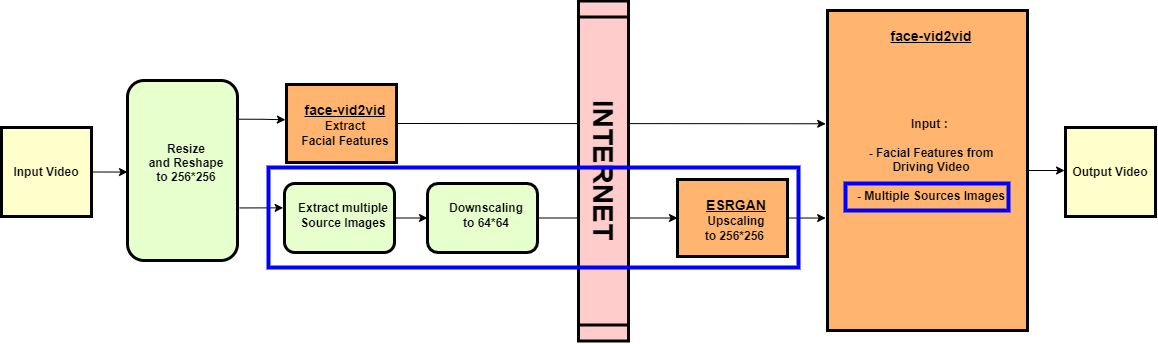
\includegraphics[width=\textwidth]{figure/ourModel.png}
    \caption{Our implemented model, the blue rectangles indicate the novelty added to the existing method \cite{Nvidia}.}
    \label{ourModel}
\end{figure*}

The aim of this project is, as mentioned in the introduction, to use a super resolution model for upscaling one or multiple source images and feed them through a talking head synthesis model to produce a video containing a talking face. 

\subsection{Talking-Head Video Synthesis Model}
For the talking-head synthesis model this paper uses an unofficial implementation of the face vid2vid model presented by NVIDIA \cite{Nvidia}.\footnote{\href{https://github.com/zhanglonghao1992/One-Shot_Free-View_Neural_Talking_Head_Synthesis}{Github for the implemented model}} This model extracts facial features from the source image as describe earlier. Then for each of those features are evaluated to extract key-points as shown by the following equations:

\begin{equation}
    x_{d,k} = R_d x_{c,k} + t_d + \delta_{d,k}
\end{equation}
\begin{equation}
    J_{d,k} = R_d J_{c,k}
\end{equation}

where J is the Jacobian matrix, R is the rotation matrix, t the translation matrix and $\delta$ is the transformation matrix. The source image's key-points are then used with the transferred video's driving key-points the flow vectors, wk’s. These flow vectors are used to warp the source features, $f_s$. The results are fed in to a motion field estimator. Then, a linear combination of the estimate flows and the motion field estimator result is applied to have our warped features fitted into the generator with the source image, to make a prediction of the frame in the video. \\

The implementation found was including pre-trained weights, trained on the VoxCeleb1 dataset.\footnote{\href{https://www.robots.ox.ac.uk/~vgg/data/voxceleb/vox1.html}{VoxCeleb1 dataset}} Since this is already trained on similar videos that will be used during inference, and training on videos is very computationally heavy, the decision was made to further try to fine tune this model. Instead it was only modified for our implementation of using multiple source images to work. This however limited our model to not be able to transfer facial features between videos (also known as deep fakes). Although a loss in feature, this was deemed as not necessary for achieving the aim of the project.

\subsection{Single Image Super Resolution Model}
A model for single-image super resolution has been implemented using Tensorflow Hub's implementation of ESRGAN. The model is trained to upscale 128x128 pixel images by 4 times, on the div2k dataset.\footnote{\href{https://data.vision.ee.ethz.ch/cvl/DIV2K/}{Div2k dataset}} This model was experimented with on the Tensorflow dataset ''aflw2k3d'', which contains images and data on faces and different facial landmarks (only the images was used).\footnote{\href{https://www.tensorflow.org/datasets/catalog/aflw2k3d}{aflw2k3d Tensorflow dataset}} The images of size 450x450 pixels was firstly downsampled to 128x128 pixels and the upsampled four times to 512x512 pixels using the model. The results from this can be seen in figure \ref{ESRGAN_comp}. When upscaling the images using this model the inference time is around 2.5 s per image (using virtual GPU in google collab). Other order of magnifications that has been tested are 1/6 and 1/8 of the original image scale. The output images was however clearly distinguishable from the original images in these cases. This might be due to the size and content of the images in the training data. In order to improve the result from this model, an attempt to fine tune the model was made by training on the previously mentioned aflw2k3d dataset. This did however not yield good enough results, due to critical color distortions and severe artifacts. This might be due to the limited computational power, only making it possible to train for one epoch with very small batch size. 
\begin{figure}[t]
  \centering
  %\fbox{\rule{0pt}{2in} \rule{0.9\linewidth}{0pt}}
   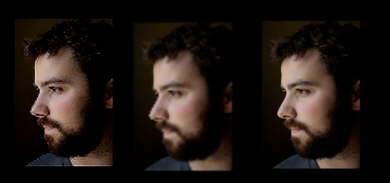
\includegraphics[scale=0.8]{figure/ESRGAN_comparison.png}

   \caption{Left: Upscaled image using Tensorflow Hub's ESRGAN implementation\\
    Middle: Image compressed to one fourth of the size and then resized to 512x512 pixels\\
    Right: Original image}
   \label{ESRGAN_comp}
\end{figure}


\subsection{Merging model}
For the first implementation of merging the different approaches, the models were sequentially executed by upscaling the first frame of the video and given as a source image for the face-vid2vid method. This was later upgraded to use multiple source images spaced out over a set interval of frames. This however resulted in a very clear transition between frames. This was especially clear when the source image deviates a lot from the driving video.\\
This is why we tried to take a new image at regular frame intervals (Figure \ref{ourModel}). We thought we could afford it since we were transmitting lower quality images which we then upscale. The main problem with this method is that if the face moves quite a bit from its initial position, we still keep sending a new image even though the ones generated have a very good quality. To avoid this problem, we tried to define a position difference threshold between the position of the initial image and the frames of the video. \\
While implementing this solution, we faced a new problem which is that when we take a new frame as source frame, we have a jump between the previous video and the current one. We tried to make the transition smoother by adding a fade-in effect for the transition which unfortunately doesn't give a better effect. We also tried to have an overlap between the two and then make the transition smoother, but this did not give us a good result.

%%%%%%%%%%%%%%%%%%%%%%%%%%%%%%%%%%%%%%%%%%%%%%%%%%%%%%%%%%%%%%%%%%%%%%
\section{Experimental results}
In this section we display the results generated by our implemented method. We found that the solution sending frames regularly at a predefined frequency provided the best results compared with the other solutions/implementations mentioned in the method section. It should be mentioned that the term "frequency" in this paper means the interval at which we send the new source-image to the generator (i.e a frequency of $10$ means that for every $10$th frame in the driving video, we will send a new source image to the generator).  We compare our resulting video with the video generated by the implementation of face-vid2vid, both with and without the ESRGAN implemented. An animated result of the comparison can be seen in figure \ref{comparison1}. It is advised to open the paper in Adobe Reader to experience the animated results. As seen in \ref{comparison1} the face-vid2vid implementation generates a video where the person in the video has closed eyes for the whole video. This is due to the source-image used in this implementation (here it was chosen at random from the driving video), where the person in this source image has her eyes closed. Our implementation is not sensitive to the single source image, because we are sending multiple source images at a predefined frequency. This effect is clearly seen in \ref{comparison1}.   \\
We also compared the difference of sending the source image to the generator at different frequencies. As seen in the animated result in \ref{Comparison2} different frequencies does not change/prevent the resulting video from "jumping" when the new source image is fed to the generator, however the amount of jumps is reduced with higher frequency. \\

Since our main goal in this paper is to synthesize a video of a talking head used for conferencing, we aim to send as less data as possible, without loosing the quality of the synthesized talking head. To achieve this task we made use of the ESRGAN, combined with the idea of sending multiple source images reduced to a lower resolution to the generator. We compare the amount of data we send in our method for different frequencies both with the face-vid2vid implementation and with the commercial H.264 standard. This comparison is shown in figure \ref{datatransmitted}. As seen in the figure already at frequencies starting from $15$ our implementation without ESRGAN transmits less amount of data than the commercial H.264. Also we see that at frequencies of $45$ and above our method is transferring less amount of data than the face-vid2vid \cite{Nvidia} implementation.   

\begin{figure}[t]
  \centering
  %\fbox{\rule{0pt}{2in} \rule{0.9\linewidth}{0pt}}
   \includesvg[scale=0.6]{figure/graph2.svg}

   \caption{Comparison of the Bytes transmitted for our method at different frequencies (here ranging from 1 to 100) for a video consisting of $600$ frames. As mentioned earlier frequency is defined as the interval at which new source image is send to the generator, hence when the frequency increases the amount of data transmitted decreases.}
   \label{datatransmitted}
\end{figure}

\section{Conclusion and Future works}
In conclusion, the final result of the model is efficient to treat the problem. It allows to have more data to send, but treats better the occlusion problems to be treated. It remains an improvement of the initial problem thanks to the ESRGAN which allows us to send less data. There still however continue to treat the teleportation problems to find a way to fix them and also try to implement the method with a distance threshold that we did not manage to fix. Maybe one way to fix the problem is to create an optical flow map to try to add one or more intermediate frames when changing to a new image to try to make the transition look smoother. More information about the project can be found on the   \href{https://github.com/FlowBigby/Super-Resolution-Multi-Shot-Neural-Talking-Head-Synthesis}{Github folder}


\begin{figure}[t]
  \centering
  %\fbox{\rule{0pt}{2in} \rule{0.9\linewidth}{0pt}}
   \animategraphics[loop,autoplay,scale=0.30]{20}{"Comparison1/DoneComparison_10frames_frame"}{0}{76}

   \caption{Animated comparison of the original face-vid2vid implementation with random source image (first frame) and our implemented method, sending source images every $10$th frame both with and without the implementation of the ESRGAN (2 last frames). (open in Adobe Reader to see animation)}
    
   \label{comparison1}
\end{figure}


\begin{figure}[t]
  \centering
  %\fbox{\rule{0pt}{2in} \rule{0.9\linewidth}{0pt}}
   \animategraphics[loop,autoplay,scale=0.30]{20}{"Comparison2/Comparison_esrgan_10_20_and_30frames_frame"}{0}{76}

   \caption{Animated comparison of the original face-vid2vid implementation with random source image (first frame) and our implemented method, sending source images every $10$th frame both with and without the implementation of the ESRGAN (2 last frames). (open in Adobe Reader to see animation)}
    
   \label{Comparison2}
\end{figure}

%%%%%%%%% REFERENCES
\newpage
{\small
    \bibliographystyle{ieee_fullname}
    \bibliography{egbib}
}

\end{document}
